%\documentclass[xcolor=table,handout,compress]{beamer}
\documentclass[xcolor=table]{beamer}
%--------------------------------------------------------------------------
% Common packages
%--------------------------------------------------------------------------
\usepackage[english]{babel}
\usepackage{pgfpages} % required for notes on second screen
\usepackage{graphicx}
\usepackage{subfigure}
\usepackage{multicol}
\usepackage[normalem]{ulem}

\usepackage{tabularx,ragged2e}
\usepackage{booktabs}
\usepackage{marvosym}

\makeatletter
\let\beamer@writeslidentry@miniframeson=\beamer@writeslidentry
\def\beamer@writeslidentry@miniframesoff{%
  \expandafter\beamer@ifempty\expandafter{\beamer@framestartpage}{}% does not happen normally
  {%else
    % removed \addtocontents commands
    \clearpage\beamer@notesactions%
  }
}
\newcommand*{\miniframeson}{\let\beamer@writeslidentry=\beamer@writeslidentry@miniframeson}
\newcommand*{\miniframesoff}{\let\beamer@writeslidentry=\beamer@writeslidentry@miniframesoff}
\makeatother


%--------------------------------------------------------------------------
% Load theme
%--------------------------------------------------------------------------
\usetheme{hri}

\usepackage{tikz}
\usetikzlibrary{patterns,shapes,fpu,fit,calc,mindmap,backgrounds,positioning,svg.path}

\tikzset{
  invisible/.style={opacity=0},
  visible on/.style={alt={#1{}{invisible}}},
  alt/.code args={<#1>#2#3}{%
    \alt<#1>{\pgfkeysalso{#2}}{\pgfkeysalso{#3}} % \pgfkeysalso doesn't change the path
  },
}

\newcommand*\circled[1]{\tikz[baseline=(char.base)]{
            \node[shape=circle,draw,inner sep=1pt] (char) {\bf\tiny #1};}}


%% Neat trick to have only one navigation bullet per subsection
%% http://tex.stackexchange.com/questions/64333/one-navigation-bullet-per-subsection-with-subsection-false-in-custom-beamer-them
%\usepackage{etoolbox}
%\makeatletter
%\patchcmd{\slideentry}{\advance\beamer@xpos by1\relax}{}{}{}
%\def\beamer@subsectionentry#1#2#3#4#5{\advance\beamer@xpos by1\relax}%
%\makeatother
%%%%%%%%%%%%%%%%%%%%%%%%%%%%%%%%%%%%%%%

\graphicspath{{figs/}}

% for model of anthopomorphism
\newcommand{\IPA}{{$\mathcal{A}_0$~}}
\newcommand{\SLA}{{$\mathcal{A}_\infty$~}}
\newcommand{\sla}{{\mathcal{A}_\infty}}
\newcommand{\AntMax}{{$\mathcal{A}_{max}$~}}
\newcommand{\antMax}{{\mathcal{A}_{max}}}

% for HATP plans
\newcommand{\hatpaction}[3]{#1\\\textsf{\scriptsize #2,}\\\textsf{\scriptsize #3}}
\newcommand{\stmt}[1]{{\footnotesize \tt  #1}}

% for mutual modelling
\newcommand{\Mmodel}[3]{{\mathcal{M}(#1, #2, #3)}}
\newcommand{\model}[3]{{$\mathcal{M}(#1, #2, #3)$}}
\newcommand{\Model}[3]{{$\mathcal{M}^{\circ}(#1, #2, #3)$}}

% typeset logical concept
\newcommand{\concept}[1]{{\scriptsize \texttt{#1}}}

\newcommand{\backbutton}{\hfill\hyperlink{appendix}{\beamerreturnbutton{Supplementary material}}}
%--------------------------------------------------------------------------
% General presentation settings
%--------------------------------------------------------------------------
\title{\Large Co-designed head to toe}
\subtitle{Towards end-to-end participatory design}
\date{{\bf RoMAN21 -- BAILAR Workshop} | 08 Aug 2021}
\author{Séverin Lemaignan}
\institute{{\bf Bristol Robotics Lab} University of the West of England \\
\emph{(soon PAL Robotics!)}}

%--------------------------------------------------------------------------
% Notes settings
%--------------------------------------------------------------------------
%\setbeameroption{show notes on second screen}
%\setbeameroption{hide notes}

\begin{document}


%%%%%%%%%%%%%%%%%%%%%%%%%%%%%%%%%%%%%%%%%%%%%%%%%%%%%%%%


%%%%%%%%%%%%%%%%%%%%%%%%%%%%%%%%%%%%%%%%%%%%%%%%%%%%%%%%

\licenseframe{github.com/severin-lemaignan/presentation-codesign}

\maketitle
\imageframe{my_background/00}




\begin{frame}<1-7>[label=soro]{Social Robotics}
    \centering

    \begin{columns}
        \begin{column}{0.7\linewidth}

            \only<1>{
                Creating interactive robots that are \textbf{embedded and
                understand their (human) social context}; \textbf{generate and adopt appropriate
                social behaviours}; have a \textbf{positive impact on human
                society}.

                \vspace{2em}
                $\Rightarrow$ designing and implementing the \textbf{assistant and
                companion robots} for  tomorrow.

                \vspace{2em}
                $\Rightarrow$ direct impact on ageing society, education, customer service;
                \textbf{major socio-economic
                challenge}
            }

            \only<2->{
                \textbf{Major scientific challenges}:

                \begin{itemize}
                    \item<2-> Model open-ended, underspecified situations; rich
                        semantics; complex social dynamics;
                    \item<3-> Close the interaction loop;
                    \item<4-> Understand and sustain long-term autonomous social interactions;
                    \item<5-> Real-world algorithmic robustness;
                    \item<6-> Complex ethical landscape;
                    \item<7-> $\Rightarrow$ cross-disciplinary \& holistic approach required
                    \item<7-> $\Rightarrow$ involve all the stakeholders;
                        participatory approach

                \end{itemize}


                \uncover<8>{
                \vspace{1em}


                \setbeamercolor{hriSec1Demo}{bg=hriSec3Dark,fg=white}
                \begin{beamercolorbox}[wd=\linewidth,ht=8ex,dp=0.7ex]{hriSec1Demo}
                    \large \bf \centering
                    Socially-Driven Autonomous Robots \\
                    for \\
                    Real-world Human-Robot Interactions
                \end{beamercolorbox}
            }


            }
        \end{column}
        \begin{column}{0.35\linewidth}
            \begin{center}
                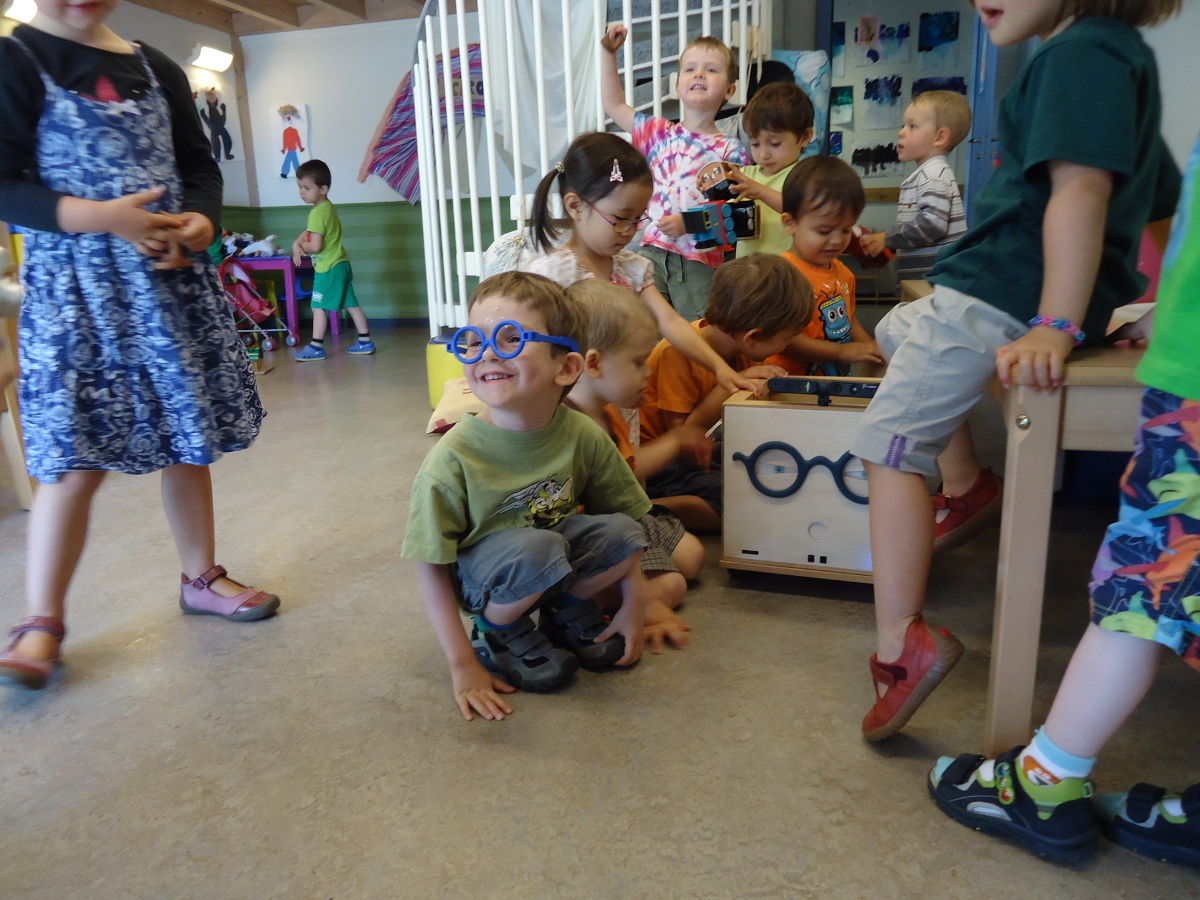
\includegraphics[trim=15cm 0 11cm 0,clip,width=\linewidth]{ranger/ranger_funny_glasses}
            \end{center}
        \end{column}
    \end{columns}

\end{frame}



\begin{frame}{Let set ourselves a challenge}

\begin{exampleblock}{Design \& run a study with:}
    
    \begin{itemize}
        \item<+-> a real robot
        \item<+-> a real interaction (...with a human!)
        \item<+-> a continuous interaction
        \item<+-> a realistic task (large state vector \& action space)
        \item<+-> in the wild
        \item<+-> also including social behaviours \& social dynamics
        \item<+-> ...and of course, the robot should be autonomous
    \end{itemize}
\end{exampleblock}

\end{frame}


\imageframe[caption=Study 1: School Tutor,color=black]{sparc/overview}

{
    \paper{Senft et al. \textbf{Teaching robots social autonomy from in situ
    human guidance} Science Robotics 2019}

\begin{frame}{IRL applied to social robotics}

    \begin{columns}
        \begin{column}{0.5\linewidth}

            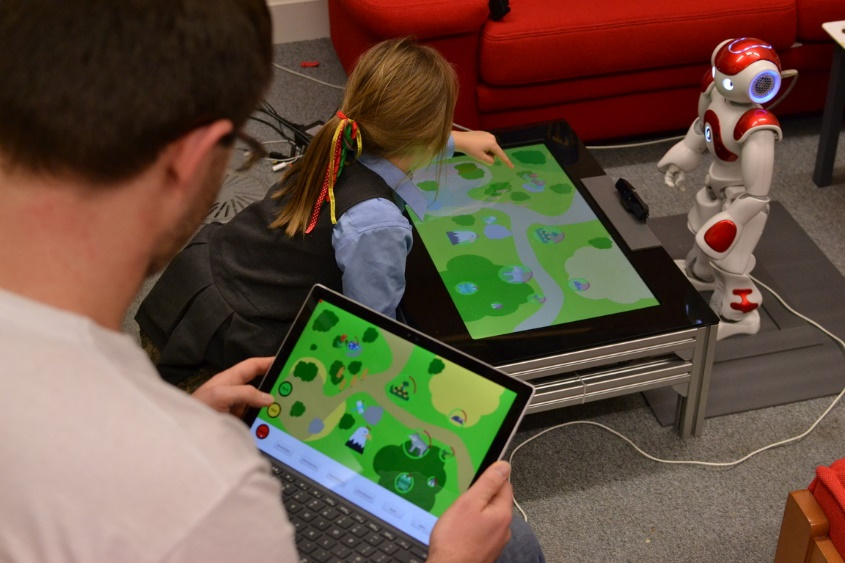
\includegraphics[width=\linewidth]{sparc/overview}

        \end{column}
        \begin{column}{0.5\linewidth}
            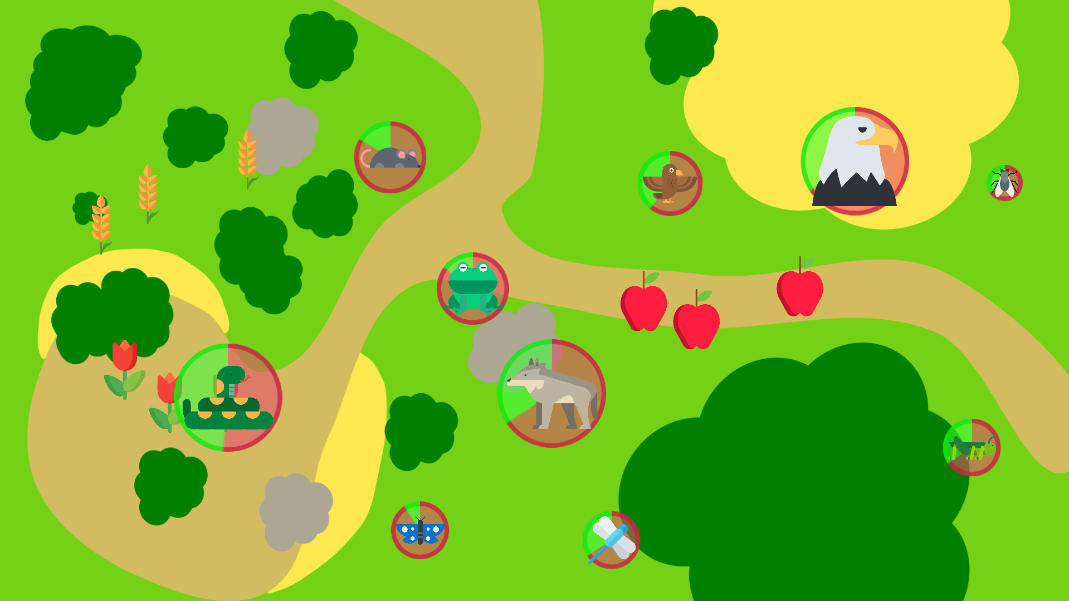
\includegraphics[width=\linewidth]{sparc/gui}
        \end{column}
    \end{columns}

    The children plays a game about food chains; the robot learns to guide them
    (\emph{task-specific action policy}) and encourage them (\emph{social action
    policy})

    Interactive Machine Learning (IRL) to teach the robot.

    $|state| = 210$ $| action\_space| = 655$

    \badge[caption=Emmanuel Senft]{colleagues/emmanuel}
\end{frame}

\videoframe[0.56]{figs/sparc/video.mp4?noaudio&autostart}

\begin{frame}{Teacher's interface}
    \begin{center}
        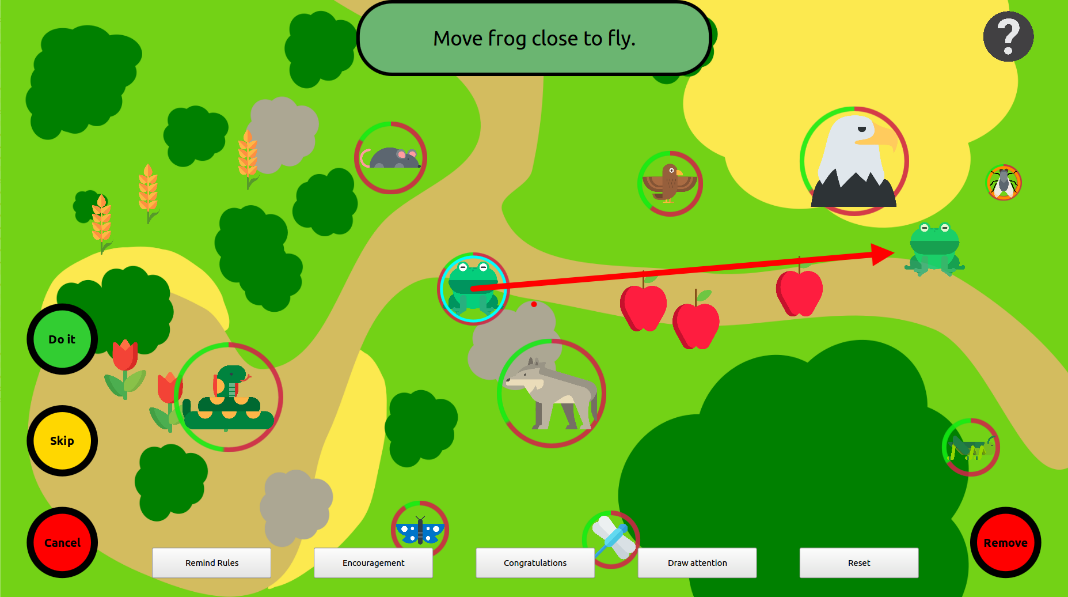
\includegraphics[width=0.9\linewidth]{sparc/woz-gui}
    \end{center}

    The robot's teacher (an end-user: might be the actual child's teacher) has a
    tablet interface that mirror's the child one, and add robot's teleoperation
    and rewards.

    \badge[caption=Emmanuel Senft]{colleagues/emmanuel}
\end{frame}


%\begin{frame}{Software architecture}
%    \begin{center}
%        \includegraphics[width=\linewidth]{figs/sparc/architecture}
%    \end{center}
%    \badge[caption=Emmanuel Senft]{colleagues/emmanuel}
%\end{frame}

%\imageframe[caption={Overall performance (pre-, mid-, post-test)},scale=0.9]{sparc/perf}

\begin{frame}{Learnt robot's behaviour}
    \only<1-2>{
        Distribution of actions for the 25 children participants:
    }
    \includegraphics<1>[width=0.9\linewidth]{sparc/actions-supervised}
    \includegraphics<2>[width=0.9\linewidth]{sparc/actions}

    \only<2>{
        $\rightarrow$ the robot personalises its action policies to the child's
        behaviour.
    }


    \only<3>{
        Time between a child's successful action and a praise:

        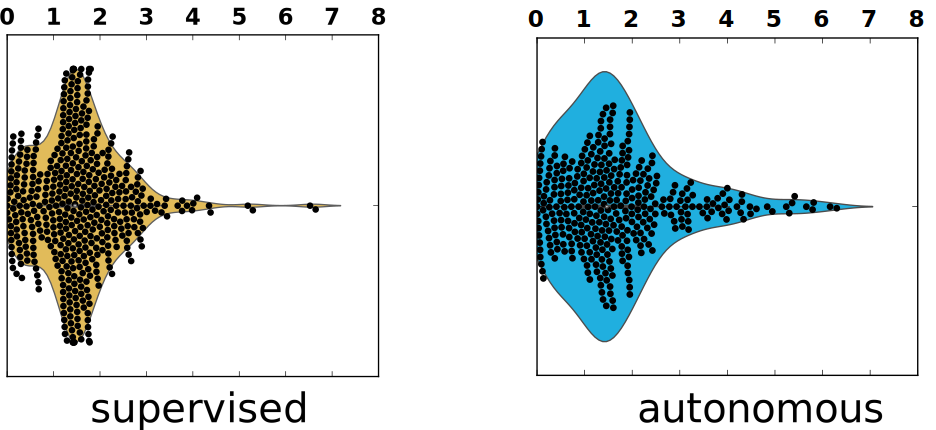
\includegraphics[width=0.9\linewidth]{sparc/social-timing}

        $\rightarrow$ the robot has also learnt an appropriate social timing.
    }

    \badge[caption=Emmanuel Senft]{colleagues/emmanuel}
\end{frame}
}


%\imageframe[color=black,caption={$|state| = 210$ $| action\_space| = 655$}]{sparc/gui}
%\imageframe[color=black]{sparc/overview}
%\videoframe[0.56]{figs/sparc/video.mp4}
%\imageframe[color=black]{sparc/woz-gui}
%\imageframe[caption={Overall performance (pre-, mid-, post-test)},scale=0.9]{sparc/perf}
%\imageframe[scale=0.9]{sparc/actions-supervised}
%\imageframe[scale=0.9]{sparc/actions}
%\imageframe[scale=0.9]{sparc/social-timing}

\begin{frame}{What does that means for the expert/teacher/end-user?}

    \begin{columns}
        \begin{column}{0.45\linewidth}
            
            \begin{center}
                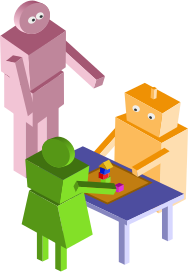
\includegraphics[width=0.9\linewidth]{sparc/sparc}
            \end{center}
        \end{column}
        \begin{column}{0.55\linewidth}
            \only<1>{
            \begin{itemize}
                \item {\bf Progressively transferring autonomy}  demonstrably
                    works in non-trivial tutoring scenarios

                \item (it also learns some elements of {\bf social behaviours} and
                    {\bf social timing})
            \end{itemize}
        }
            \only<2>{
                Key properties:

            \begin{itemize}
                \item \textbf{progressive autonomy} yet
                    \textbf{transparency} of the behaviour;
                \item \textbf{observability} and possibility to \textbf{take
                    over};
                \item because the training takes place in-situ, the
                    robot behaviours are \textbf{co-constructed} by the
                    teacher and the child
                \item $\Rightarrow$ interesting properties from a
                    ethics/responsible AI perspective
            \end{itemize}
        }
            \only<3>{
                Yet:

            \begin{itemize}
                \item Design of the input state tricky and largely task
                    dependent;
                \item What about more complex social behaviours?
                \item Would that sustain long-term interactions?
            \end{itemize}
            }
        \end{column}
    \end{columns}


\end{frame}


\imageframe[caption=Study 2: gym coach]{couch25k/hri.jpg}

{
    \paper{Winkle et al. \textbf{In-Situ Learning from a Domain Expert for Real World Socially Assistive Robot Deployment} RSS 2020}

\begin{frame}{Couch-to-5k study}

    \vspace{0.2cm}

    \begin{columns}
        \begin{column}{0.5\linewidth}
                \centering
                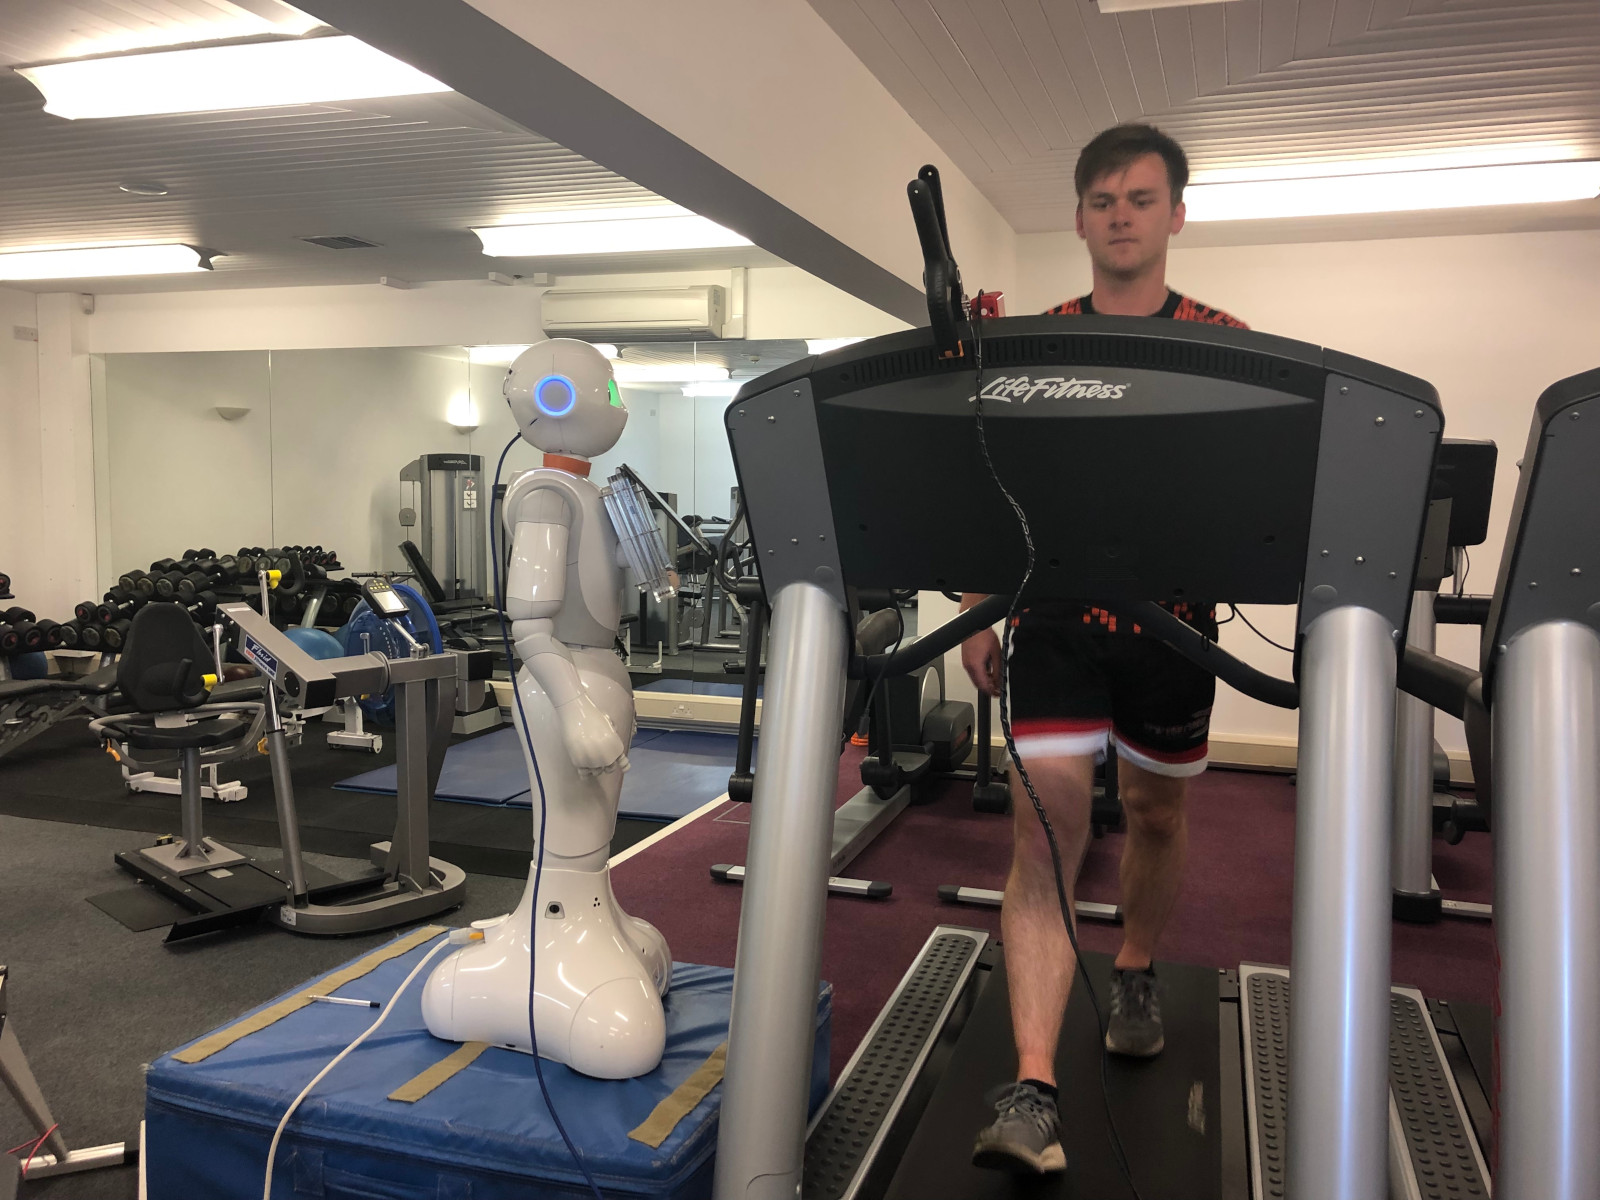
\includegraphics[height=3cm]{couch25k/hri.jpg}
        \end{column}
        \begin{column}{0.5\linewidth}
                \centering
                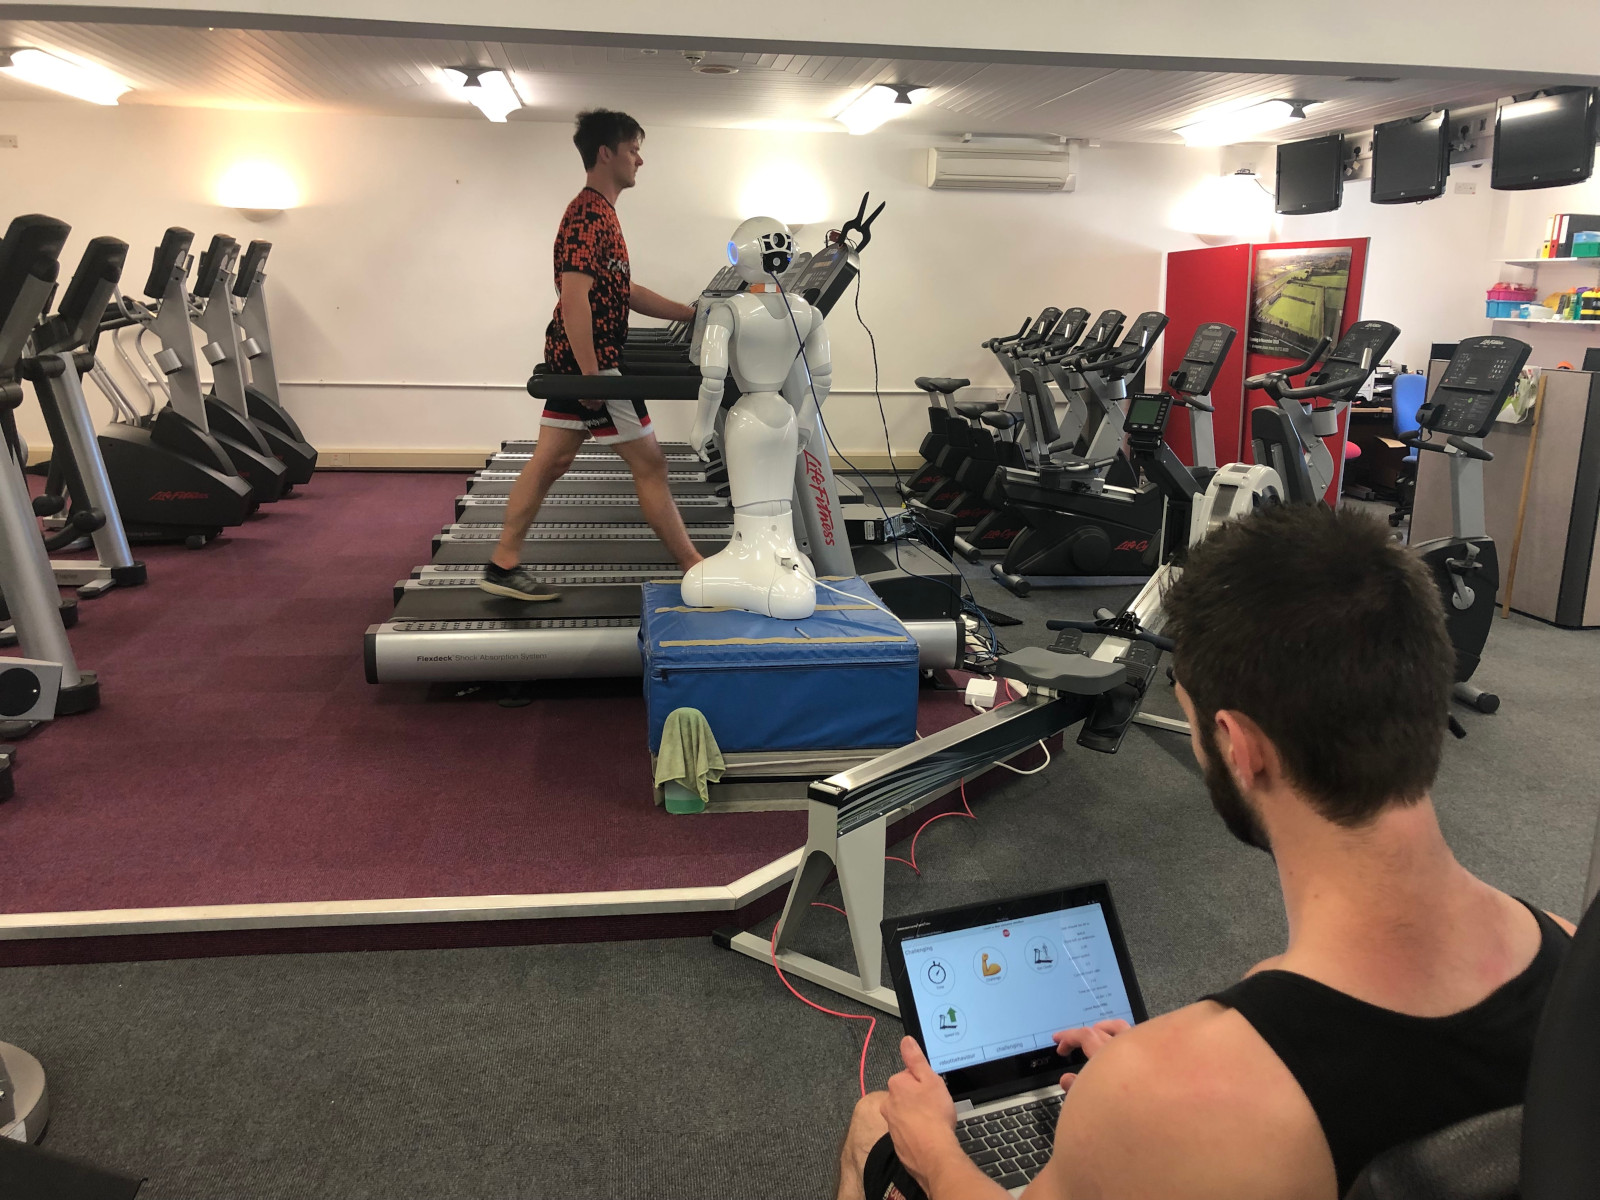
\includegraphics[height=3cm]{couch25k/supervised.jpg}
        \end{column}
    \end{columns}

    \only<1>{
    \begin{itemize}
        \item 9 participants
        \item 3 months; 27 one-hour sessions per participants
        \item $|state| = 20$ $|action\_space| = 11$
        \item Includes participants' personality (Big-5) as input feature
    \end{itemize}
    
    }

    \only<2>{
        \centering
        \includegraphics[height=4cm]{couch25k/architecture.pdf}
    }

    \badge[caption=Katie Winkle]{colleagues/katie}
\end{frame}
}

\imageframe[scale=0.9]{DesignProcess}

{
    \paper{Winkle et al. \textbf{In-Situ Learning from a Domain Expert for Real World Socially Assistive Robot Deployment} RSS 2020}

\begin{frame}{Co-design for real-world + long-term}

    \begin{center}
        \vspace{-0.7cm}
        \begin{tikzpicture}
            \node at (0,0) {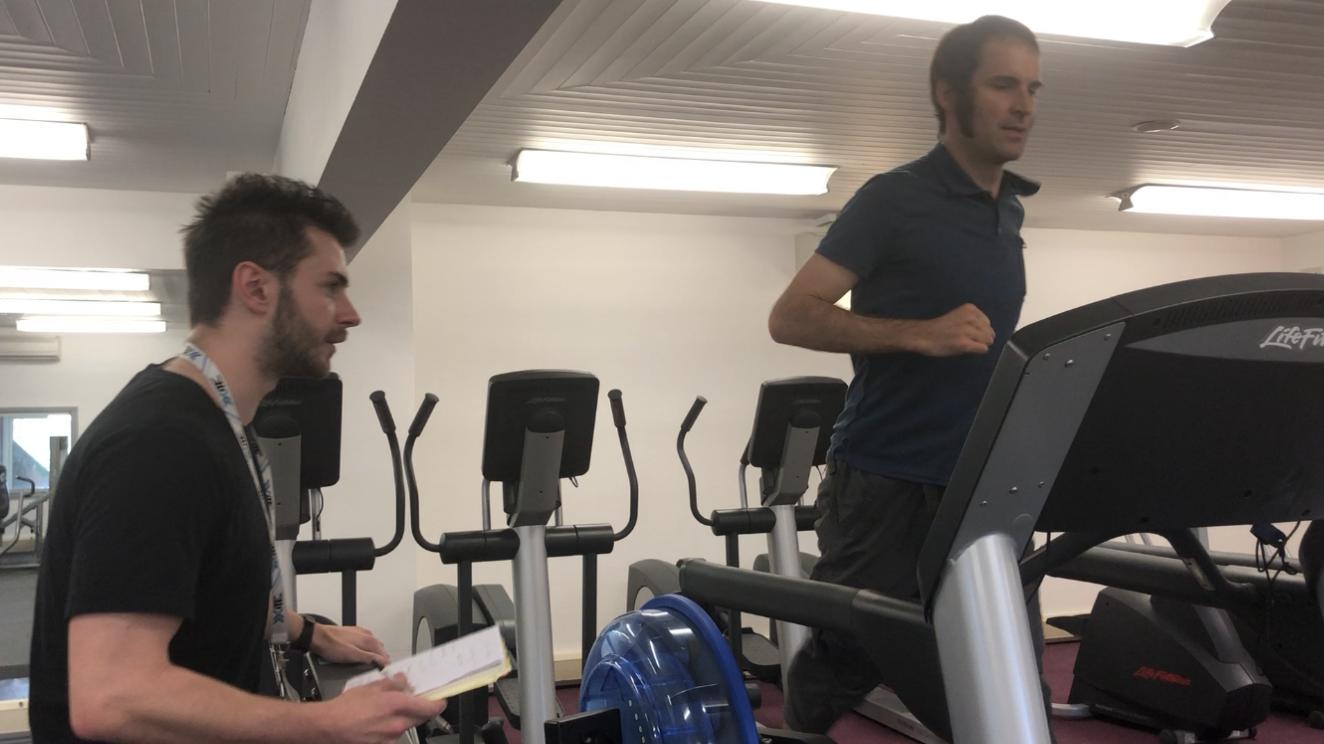
\includegraphics[width=0.6\linewidth]{figs/couch25k/couch25km-mock.jpg}};
           \node[anchor=north] at (5,0.5) {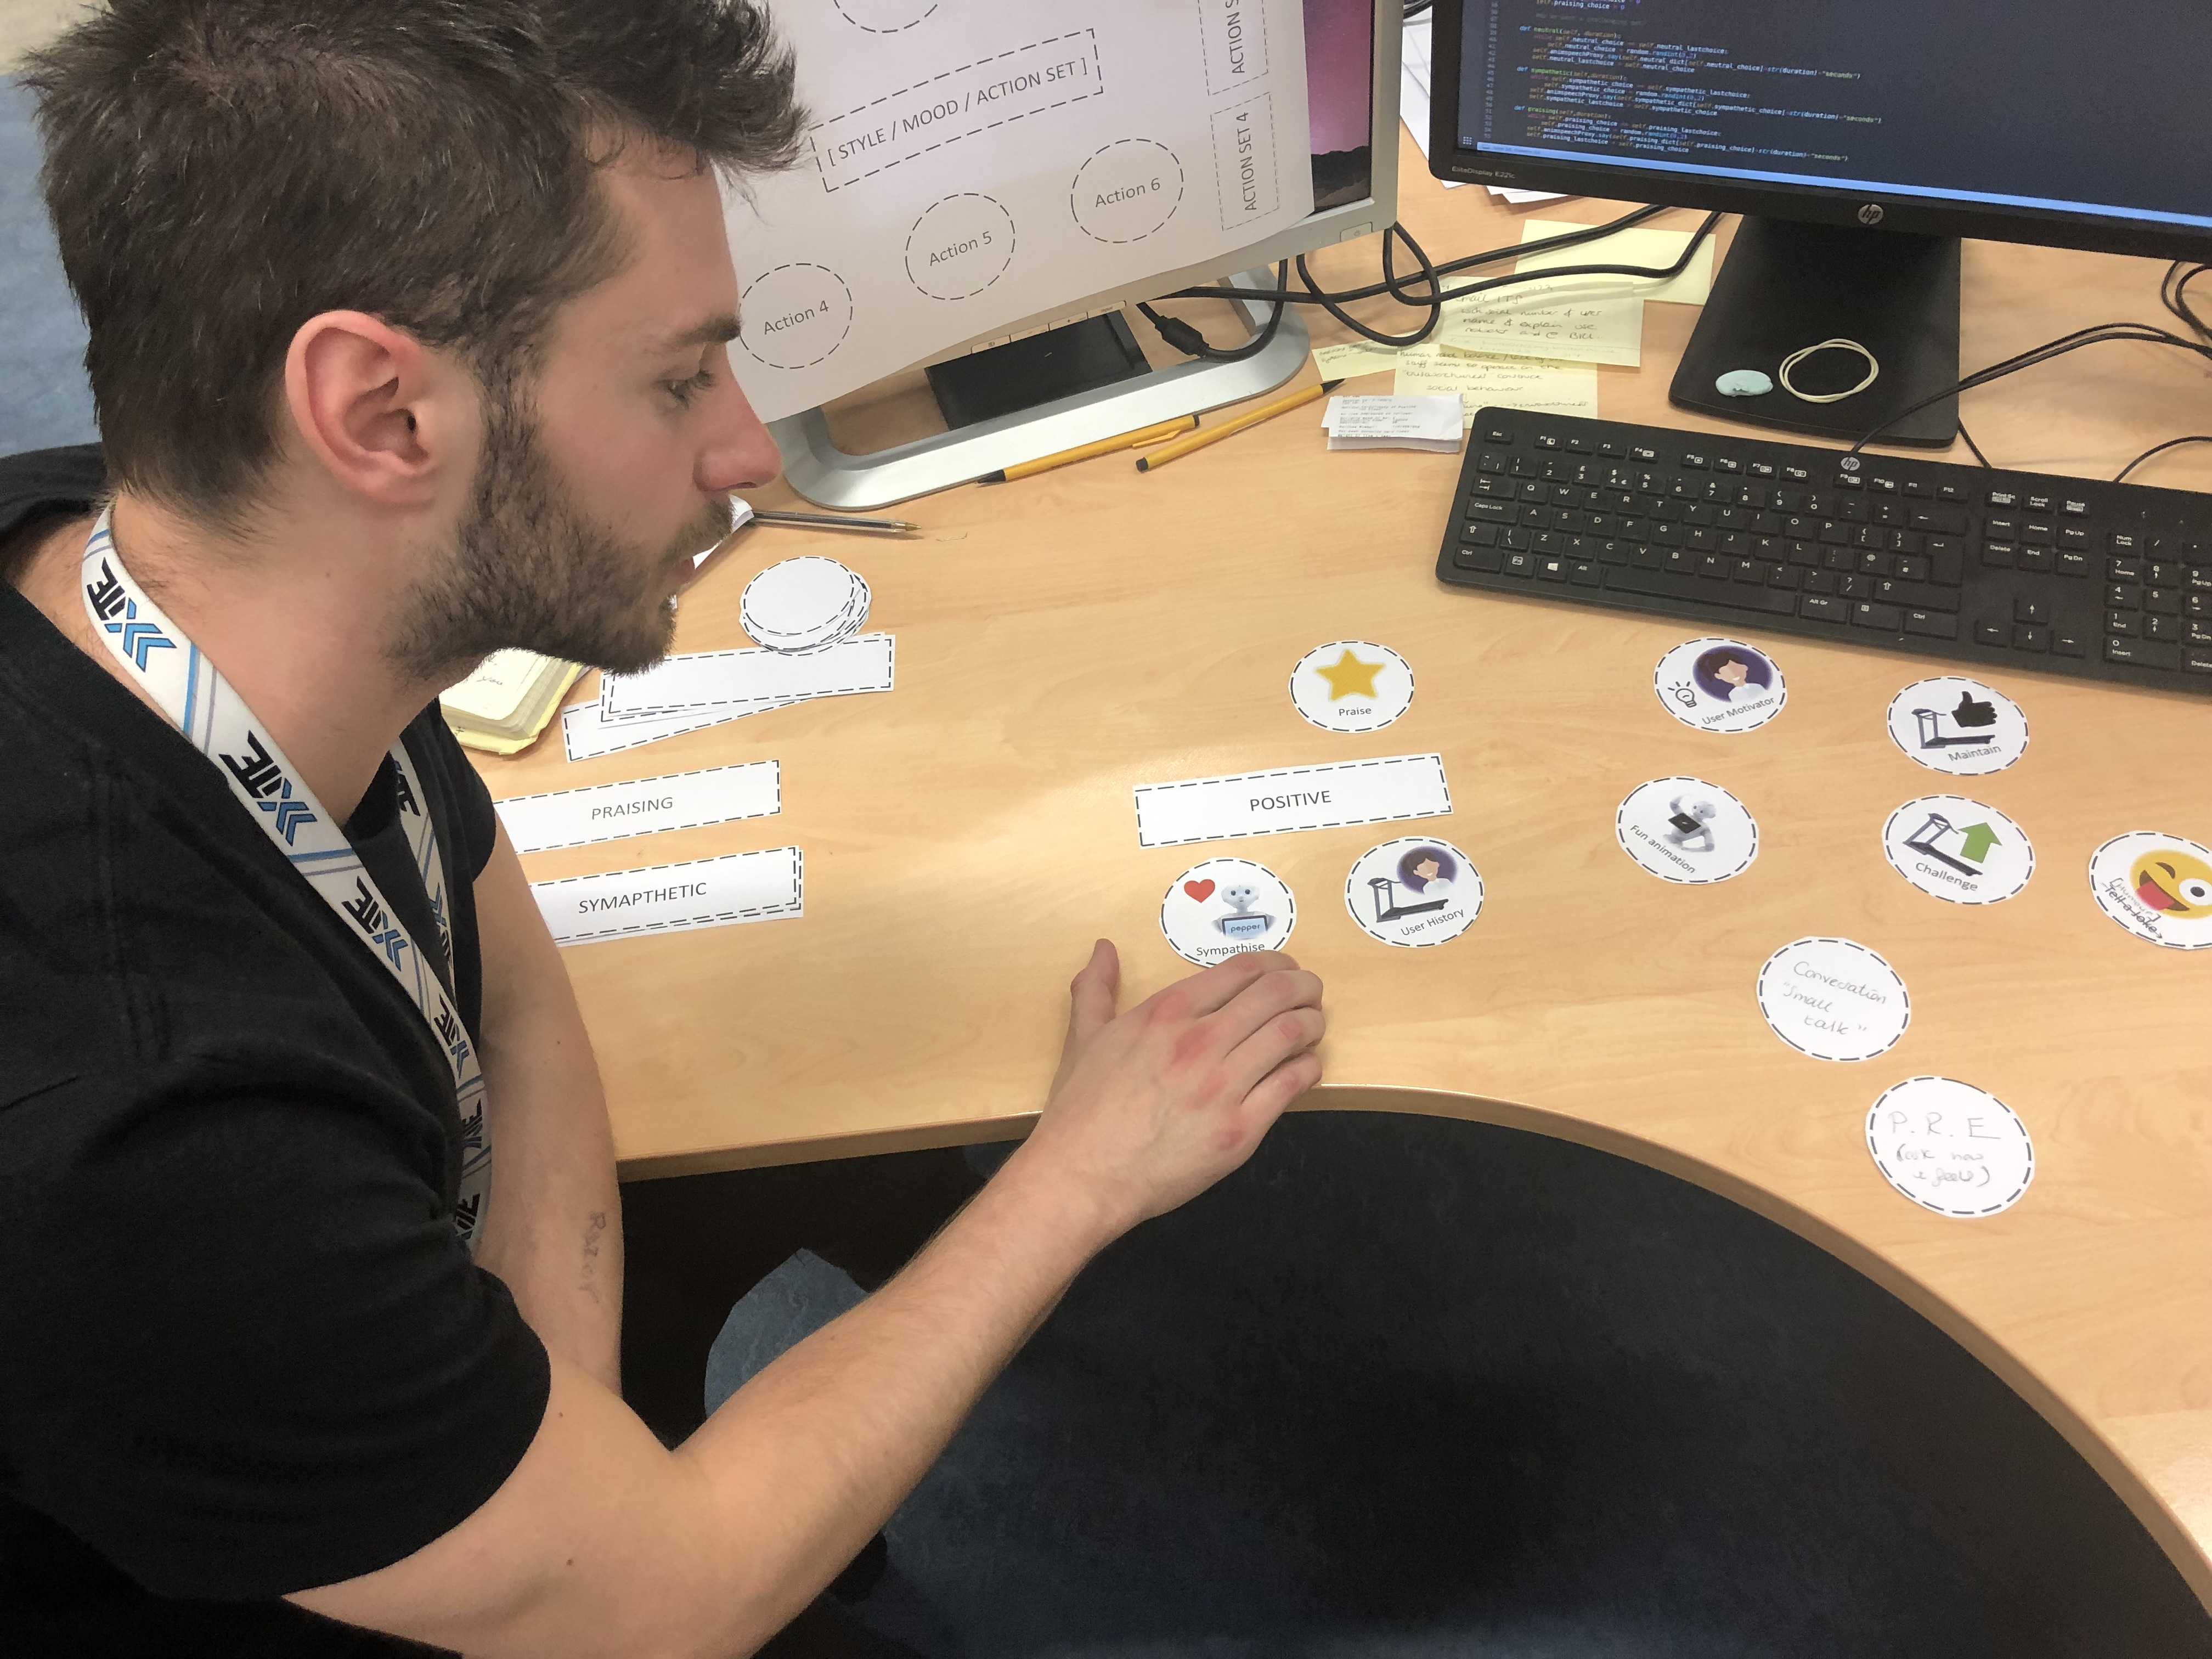
\includegraphics[trim=0 15cm 0 0,clip,width=0.6\linewidth]{figs/couch25k/codesign.jpg}};
           \node[anchor=north] at (0.5,-1.5) {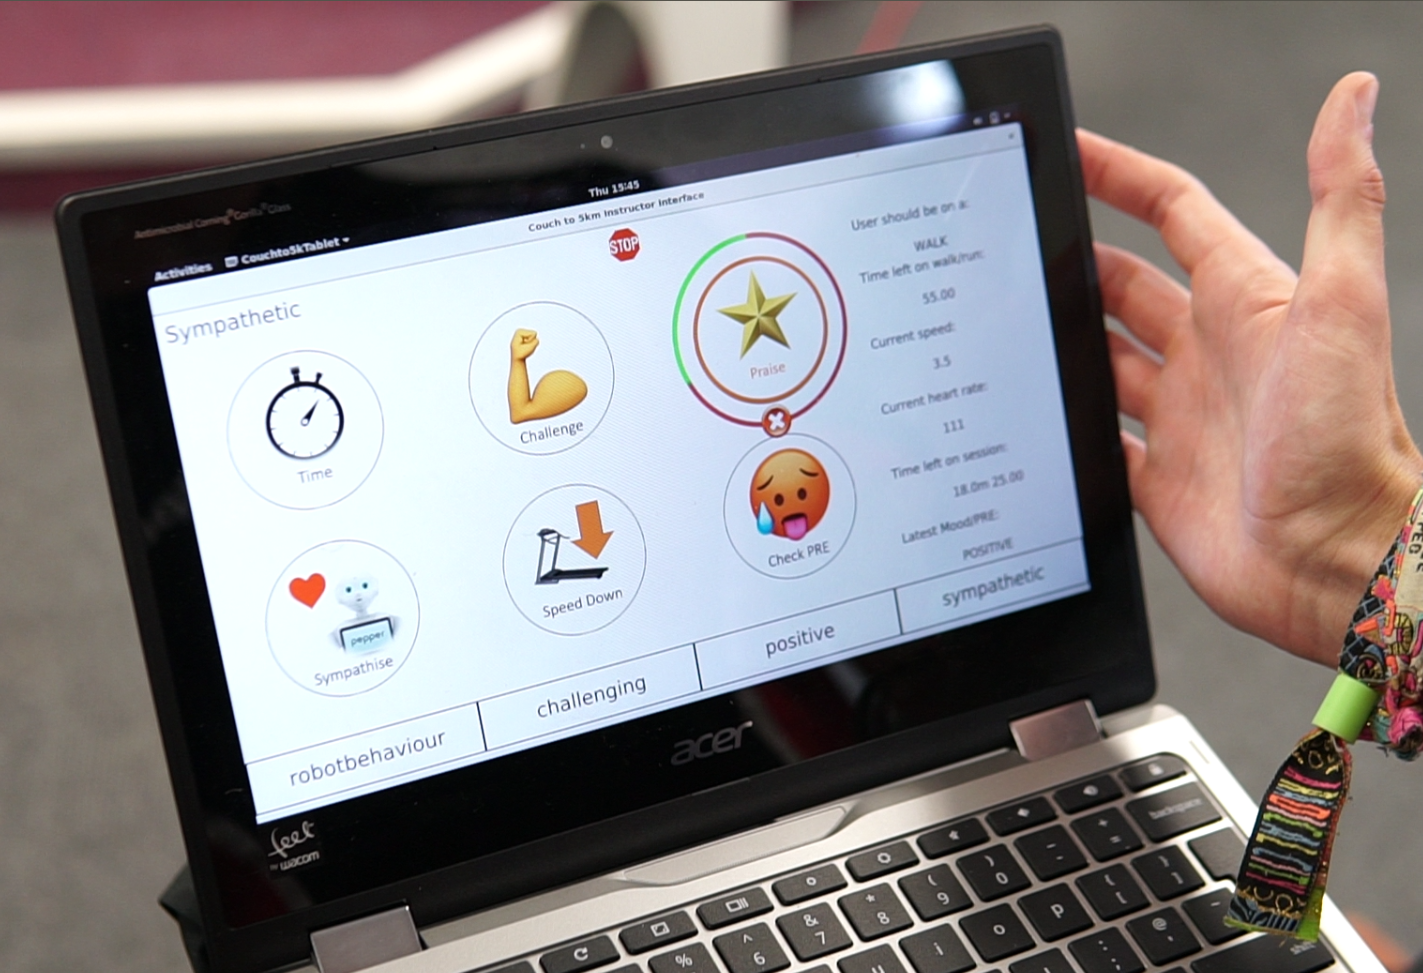
\includegraphics[width=0.5\linewidth]{figs/couch25k/teacher-ui.png}};
        \end{tikzpicture}

    \end{center}
    \badge[caption=Katie Winkle]{colleagues/katie}
\end{frame}
}



\begin{frame}{Input \& output spaces: mostly task-specific}

\only<1-2>{
  \resizebox{\linewidth}{!}{
  \begin{tabular}{|l|l|l|l|}
    \hline
    \textbf{Type} & \textbf{Feature} & \textbf{Values} & \textbf{Description} \\
    \hline
    \textbf{(Dynamic)} & Task Action Type & 0, 0.5, 1 & Whether participant is in warm-up, walk or run\\
    \textbf{Task State} & Session Progress & 0-1 & Time spent in session/session duration\\
    & Programme Progress & 0-1 & Time spent on programme/programme duration\\
    & Programme Action Progress & 0-1 & Time spent on current walk or run action/action duration\\
    & Programme Action Duration & 0, 0.5, 1 & Current walk/run action length as $\leq$ 3 mins, $\geq$ 20 mins or other\\
    & Time Since Last Action & 0-1 & Time since last action/60; capped at 1\\
    \hline
    \textbf{Dynamic} & Relative Speed: Average & 0-1 & Current speed/(2 x average speed)\\
    \textbf{Performance} & Relative Speed: Best & 0-1 & Current speed/(2 x personal best speed)\\
    \hline
    \textbf{Dynamic} & Heart Rate & 0-1 & Heart rate/2x resting heart rate capped at 1\\
    \textbf{Engagement} & Motivation/Effort & 0, 0.5, 1 & Self-reported measure in warmup/on check PRE action\\
    & Facial Expression: Lip Pull*  & 0-1 & Normalised action unit returned by OpenFace \\
    & Facial Expression: Mouth Open* & 0-1 &  Normalised action unit returned by OpenFace \\
    \hline
      \textbf{Static} & \textbf<2>{Elaboration level (self)} & 0-1 & Normalised sum of 3 Likert questions \\
      \textbf{Engagement} & \textbf<2>{Elaboration level (expert)} & 0-1 & as above but rated by fitness instructor \\
      & \textbf<2>{Activity Level} & 0-1 & Likert question response\\
    \hline
      \textbf{Static} & \textbf<2>{Extroversion} & 0-1 & Big Five measure normalised with respect to max score\\
      \textbf{Personality} & \textbf<2>{Agreeableness} & 0-1 & Big Five measure normalised with respect to max score\\
      & \textbf<2>{Conscientiousness} & 0-1 & Big Five measure normalised with respect to max score\\
      & \textbf<2>{Emotional Stability} & 0-1 & Big Five measure normalised with respect to max score\\
      & \textbf<2>{Openness to Experience} & 0-1 & Big Five measure normalised with respect to max score\\
  \hline
\end{tabular}
}

    {\tiny Features followed by * were ultimately removed due to unreliable
    detection}. \only<2>{\tiny\bf Non-task specific features.}
}
    \only<3->{

Full listing of actions as \textit{\{action-type, style-modifier\}}:

\resizebox{1.05\linewidth}{!}{
\begin{tabular}{l|l|l|l|l|l|l|l|l|l|l|l|}
\cline{2-12}
                                                         & \multicolumn{8}{c|}{\cellcolor[HTML]{FFFFC7}\textbf{Social-Supporting Actions}}                                                                                                                                                                                                                                                                                                      & \multicolumn{2}{c|}{\cellcolor[HTML]{C7EFC6}\textbf{Task Actions}}           & \multicolumn{1}{c|}{\cellcolor[HTML]{ECF4FF}\textbf{Low Level}} \\ \cline{2-12} 
                                                         & \cellcolor[HTML]{FFFC9E}\textbf{Time} & \cellcolor[HTML]{FFFC9E}\textbf{Social}                        & \cellcolor[HTML]{FFFC9E}\textbf{Performance} & \cellcolor[HTML]{FFFC9E}\textbf{Reward} & \cellcolor[HTML]{FFFC9E}\textbf{Check User} & \cellcolor[HTML]{FFFC9E}\textbf{Animation} & \cellcolor[HTML]{FFFC9E}\textbf{Get Closer} & \cellcolor[HTML]{FFFC9E}\textbf{Back Off} & \cellcolor[HTML]{9AFF99}\textbf{Run} & \cellcolor[HTML]{9AFF99}\textbf{Walk} & \cellcolor[HTML]{DAE8FC}\textbf{Eye Colour}                     \\ \hline
\multicolumn{1}{|l|}{\cellcolor[HTML]{32CB00}\textbf{P}} & Time                                  & Humour                                                         & Maintain                                     & Praise                                  & -                                           & Animation                                  & -                                           & -                                         & Run                                  & Walk                                  & Green                                                           \\ \hline
\multicolumn{1}{|l|}{\cellcolor[HTML]{F8A102}\textbf{C}} & Time                                  & Challenge                                                      & Speed Up                                     & -                                       & -                                           & -                                          & -                                           & -                                         & Run                                  & Walk                                  & Yellow                                                          \\ \hline
\multicolumn{1}{|l|}{\cellcolor[HTML]{FFCCC9}\textbf{S}} & Time                                  & \begin{tabular}[c]{@{}l@{}}Challenge\\ Sympathise\end{tabular} & Speed Down                                   & Praise                                  & Check PRE                                   & -                                          & -                                           & -                                         & Run                                  & Walk                                  & Blue                                                            \\ \hline
\multicolumn{1}{|l|}{\textbf{N}}                         & -                                     & -                                                              & -                                            & -                                       & -                                           & -                                          & Get Closer                                  & Back Off                                  & Run                                  & Walk                                  & White                                                           \\ \hline
\end{tabular}
}

{\tiny Style modifiers: P = Positive; C = Challenging; S = Sympathetic; N = Neutral.}
    }

\end{frame}




{
    \paper{Winkle et al. \textbf{In-Situ Learning from a Domain Expert for Real World Socially Assistive Robot Deployment}
    RSS 2020}
    \begin{frame}{Learnt policies}
        \begin{center}
            \includegraphics<1>[width=\linewidth]{figs/couch25k/finalactiondist-no-autonomous.png}
            \includegraphics<2>[width=\linewidth]{figs/couch25k/finalactiondist.png}
            \includegraphics<3>[width=\linewidth]{figs/couch25k/fullcomp_lbmr.pdf}
        \onslide<2>{
            (another nail in the expert systems coffin!)
        }
        \end{center}
\end{frame}
}


{
    \paper{Senft at al. \textbf{SPARC: Supervised progressively autonomous
robot competencies}, ICSR 2015;\newline
    Winkle, Senft, Lemaignan \textbf{LEADOR: End-to-End Participatory
    Design of Autonomous Social Robots} FrontiersIn 2021 (to appear)}
\begin{frame}{LEADOR: end-to-end participatory methodology}

    In retrospect:

    \begin{itemize}
        \item a successful technical solution to replace the wizard;
        \item but equally important, a \textbf{end-to-end} participatory design
            methodology
    \end{itemize}

    \pause

        From a technique:
        \begin{center}
        \textbf{SPARC: Supervised progressively autonomous robot
        competencies}
        \end{center}

        to a methodology: 
        \begin{center}
        \textbf{LEADOR: Led-by-Experts Automation and Design Of Robots}
        \end{center}


\end{frame}
}




\begin{frame}{Let's revisit our challenge}

    \begin{columns}
        \begin{column}{0.5\linewidth}

            \begin{exampleblock}{Studies with...}

                \begin{itemize}
                    \item<+->[\checkmark] real robots
                    \item<+->[\checkmark] real interactions with humans
                    \item<+->[\checkmark] continuous interactions
                    \item<+->[\checkmark] realistic tasks (large state vector \& action space)
                    \item<+->[\checkmark] in the wild
                    \item<+->[\checkmark] including social behaviours \& social dynamics
                    \item<+->[\checkmark] autonomous robot
                \end{itemize}

            \end{exampleblock}

        \end{column}
        \begin{column}{0.5\linewidth}

            \onslide<+->{
\begingroup
\setbeamercolor{block title}{bg=hriSec2Dark}
\setbeamercolor{block body}{bg=hriSec2}
            \begin{block}{End of the road:}

                \begin{itemize}
                    \item<+->[\circled{?}] open-ended, underspecified situations
                    \item<+->[\circled{?}]  rich semantics
                    \item<+->[\circled{?}]  complex social dynamics (incl. groups)
                    \item<+->[\circled{?}]  close the ``interaction loop''
                    \item<+->[$\sim$]  sustain long-term autonomous social interactions
                    \item<+->[$\sim$]  real-world robustness

                \end{itemize}
            \end{block}
\endgroup
}
        \end{column}
    \end{columns}


\end{frame}

\imageframe[color=black,caption=Study 3: robots4SEN]{figs/robots4sen/image1.jpeg}
\begin{frame}{Well-being and autism}
    \begin{columns}
        \begin{column}{0.5\linewidth}
            \begin{center}
                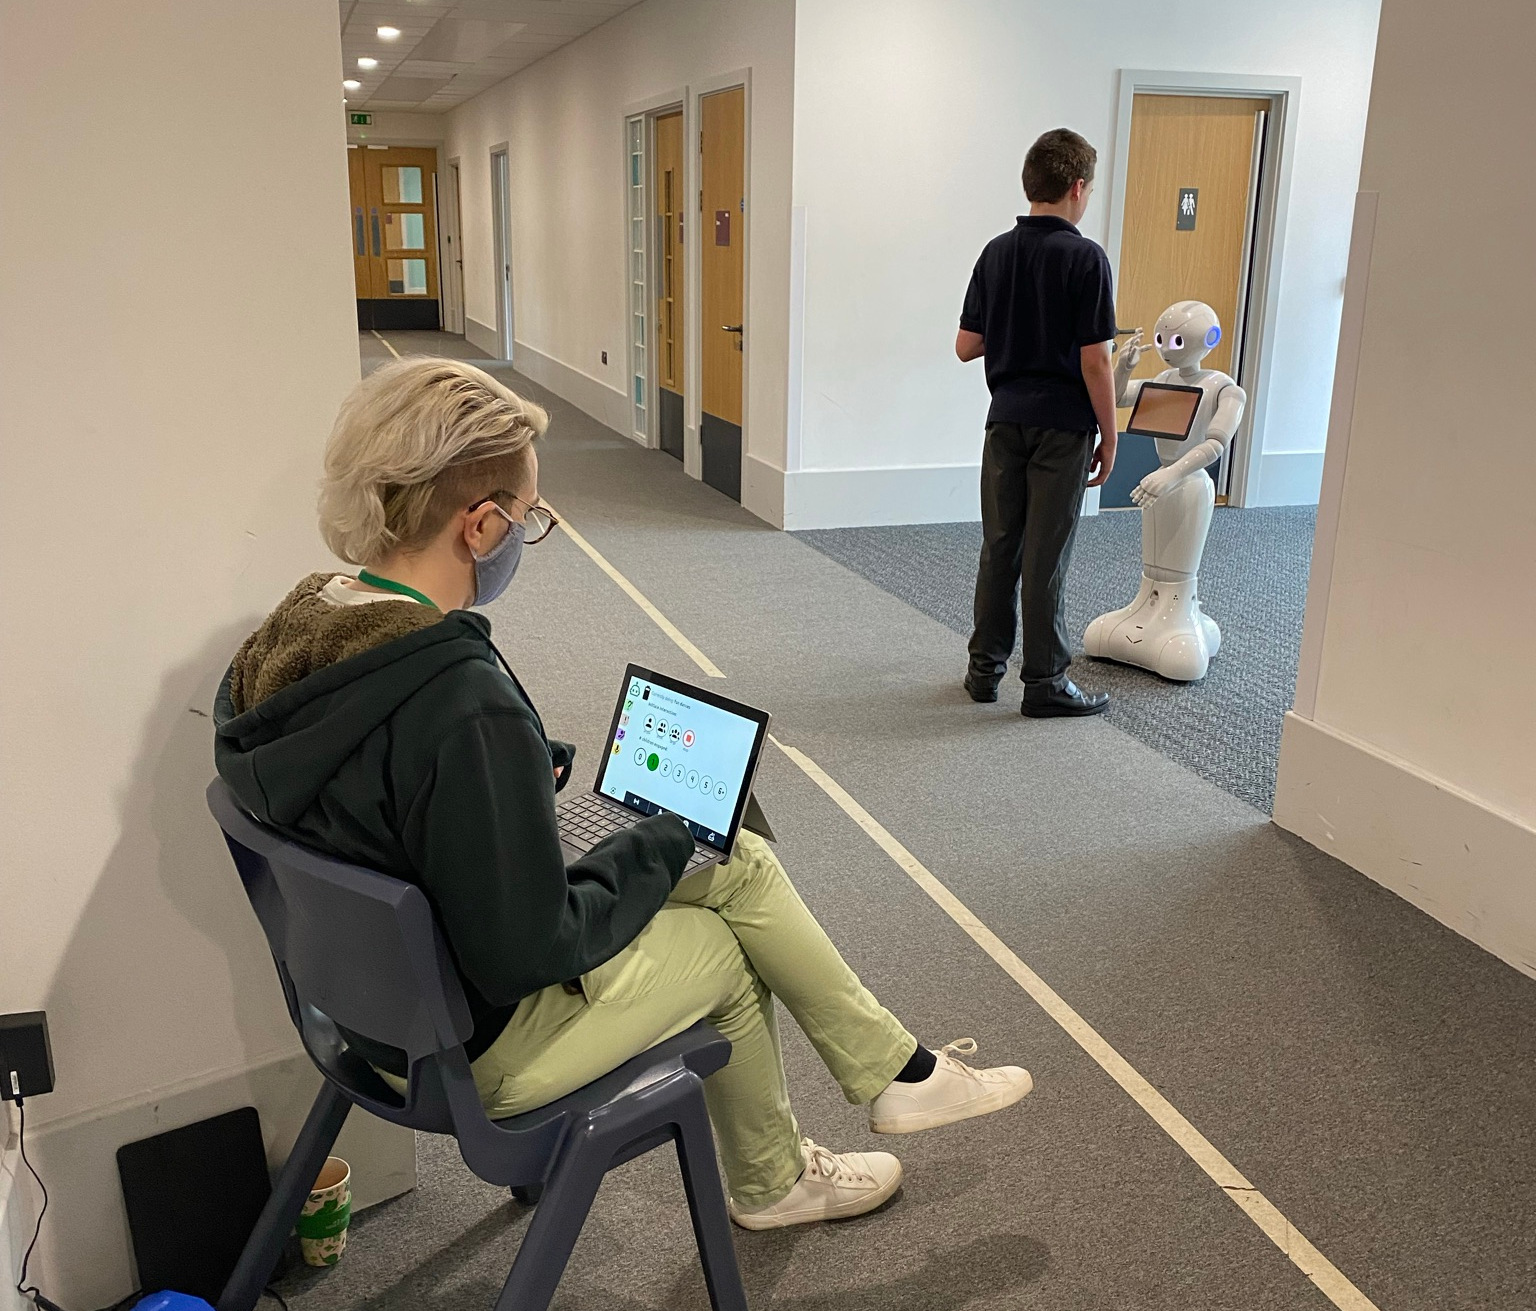
\includegraphics[width=\linewidth]{figs/robots4sen/location.jpg}
            \end{center}
        \end{column}
        \begin{column}{0.5\linewidth}
            \begin{center}
                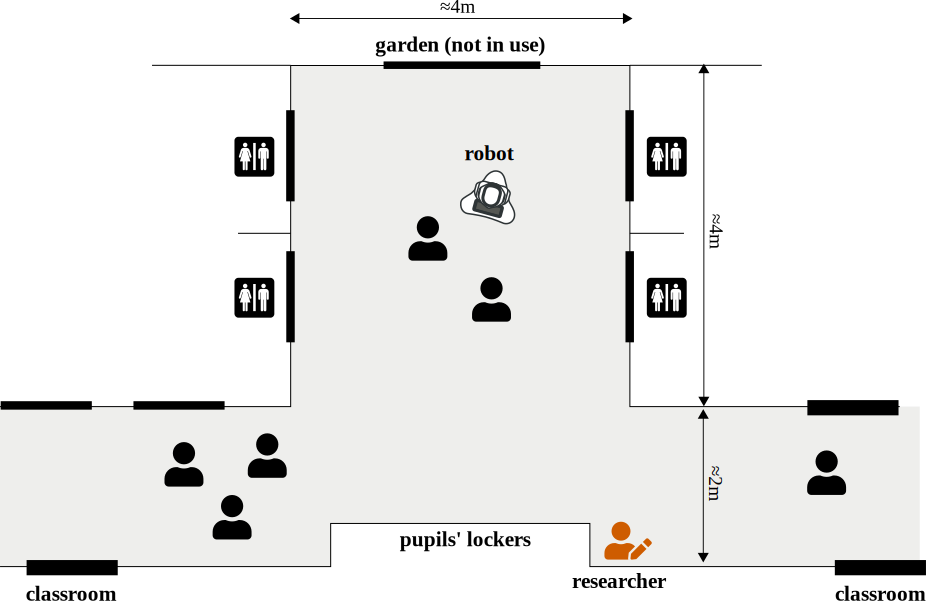
\includegraphics[width=\linewidth]{figs/robots4sen/setup}
            \end{center}
        \end{column}
    \end{columns}
\end{frame}

\begin{frame}{Participatory design with autistic children}

    \begin{center}
        \vspace{-0.7cm}
        \begin{tikzpicture}
            \node at (0,0)
            {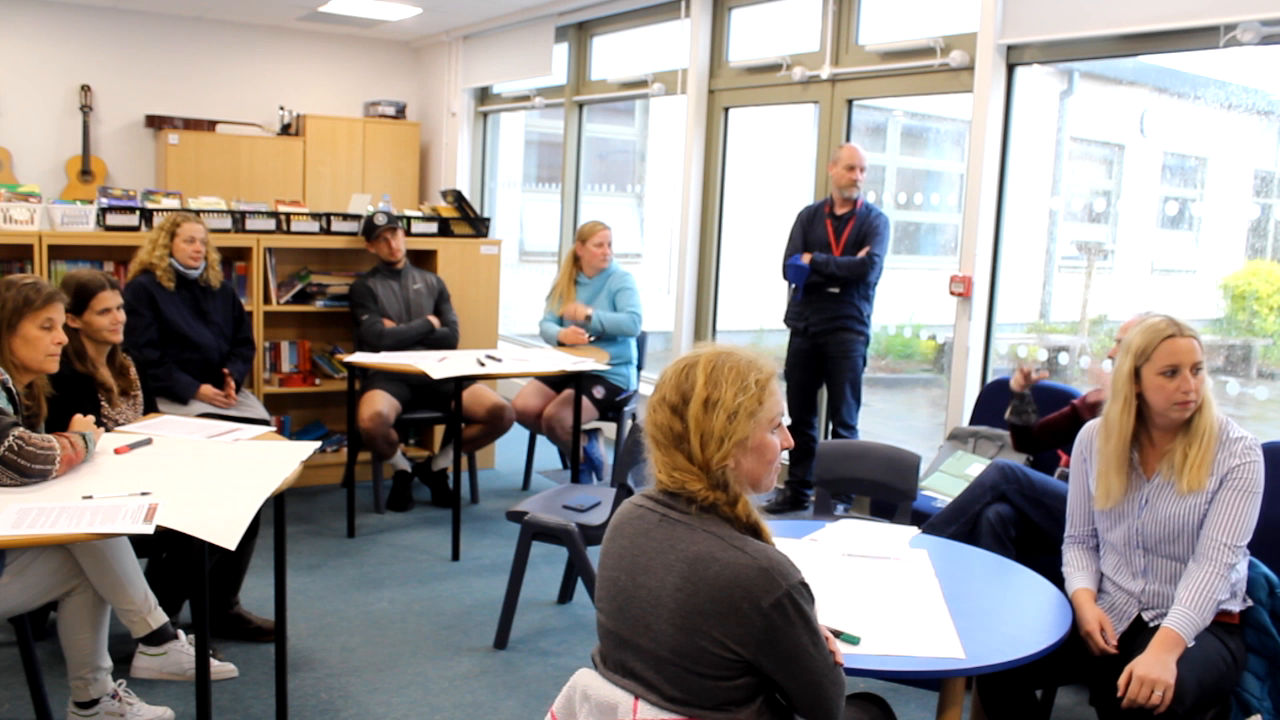
\includegraphics[width=0.6\linewidth]{figs/robots4sen/image10.png}};
           \node[anchor=north] at (5,0.)
            {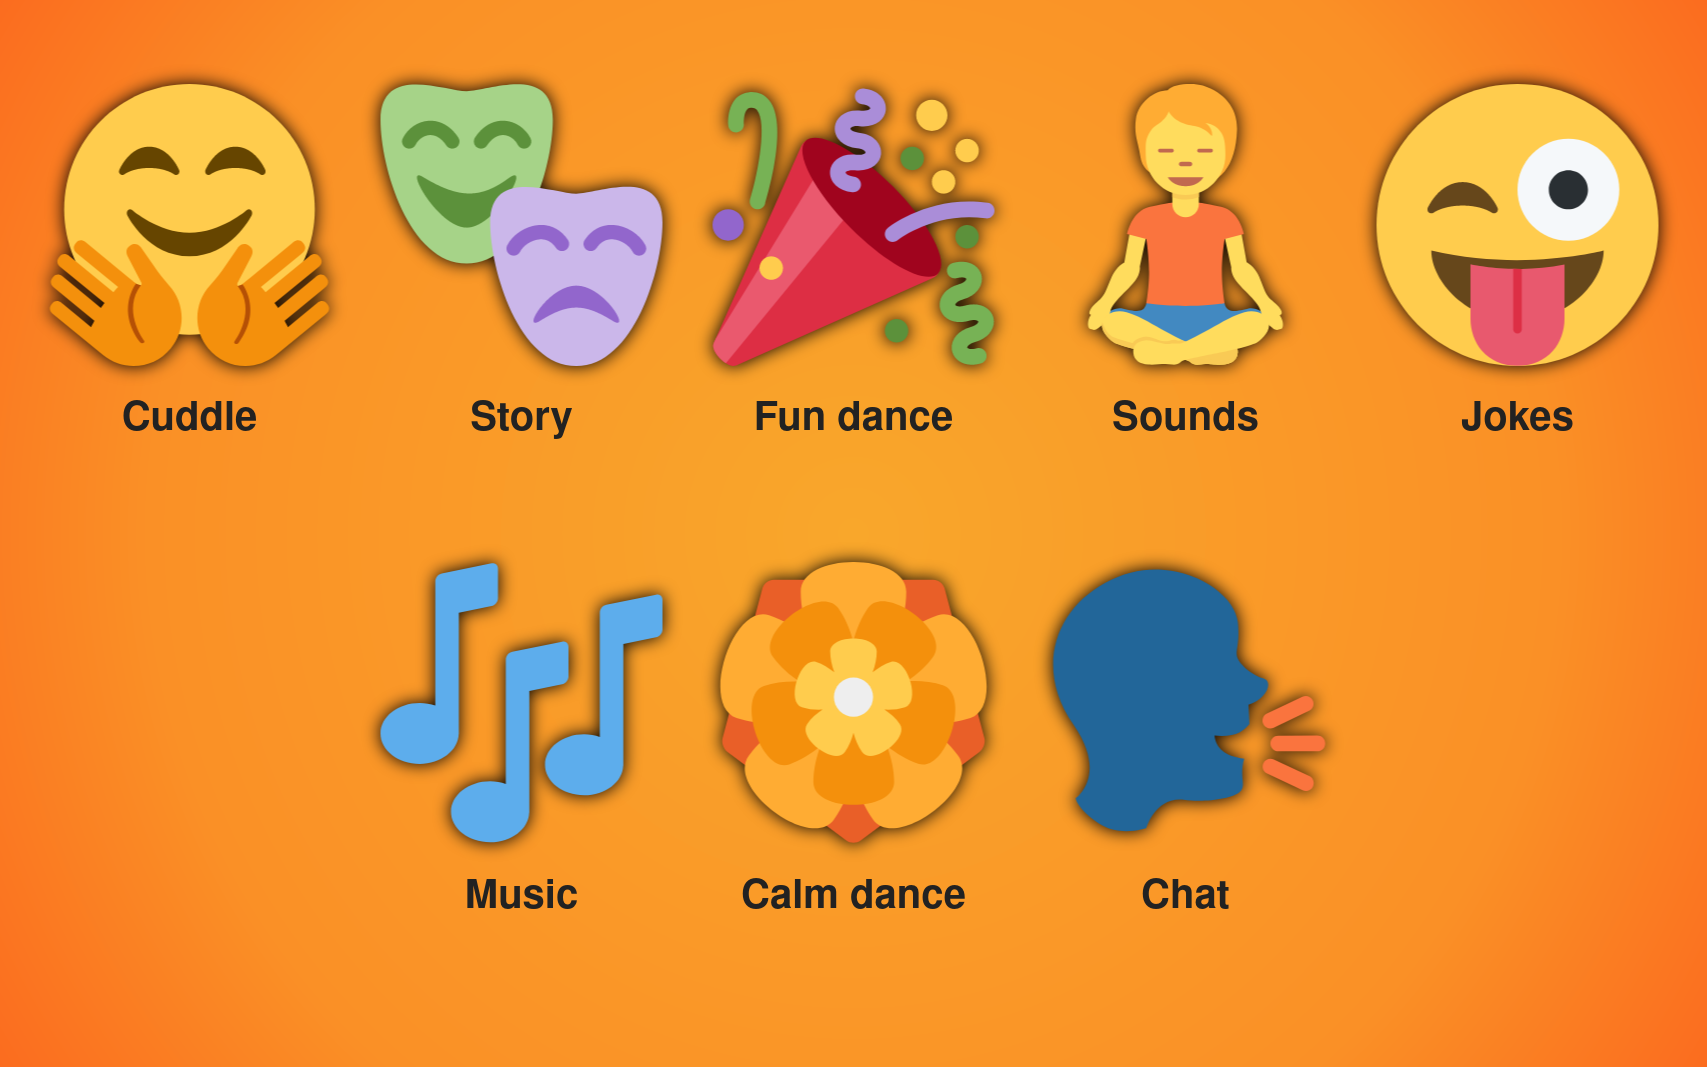
\includegraphics[width=0.5\linewidth]{figs/robots4sen/activities.png}};
           \node[anchor=north] at (0.5,-1.5)
            {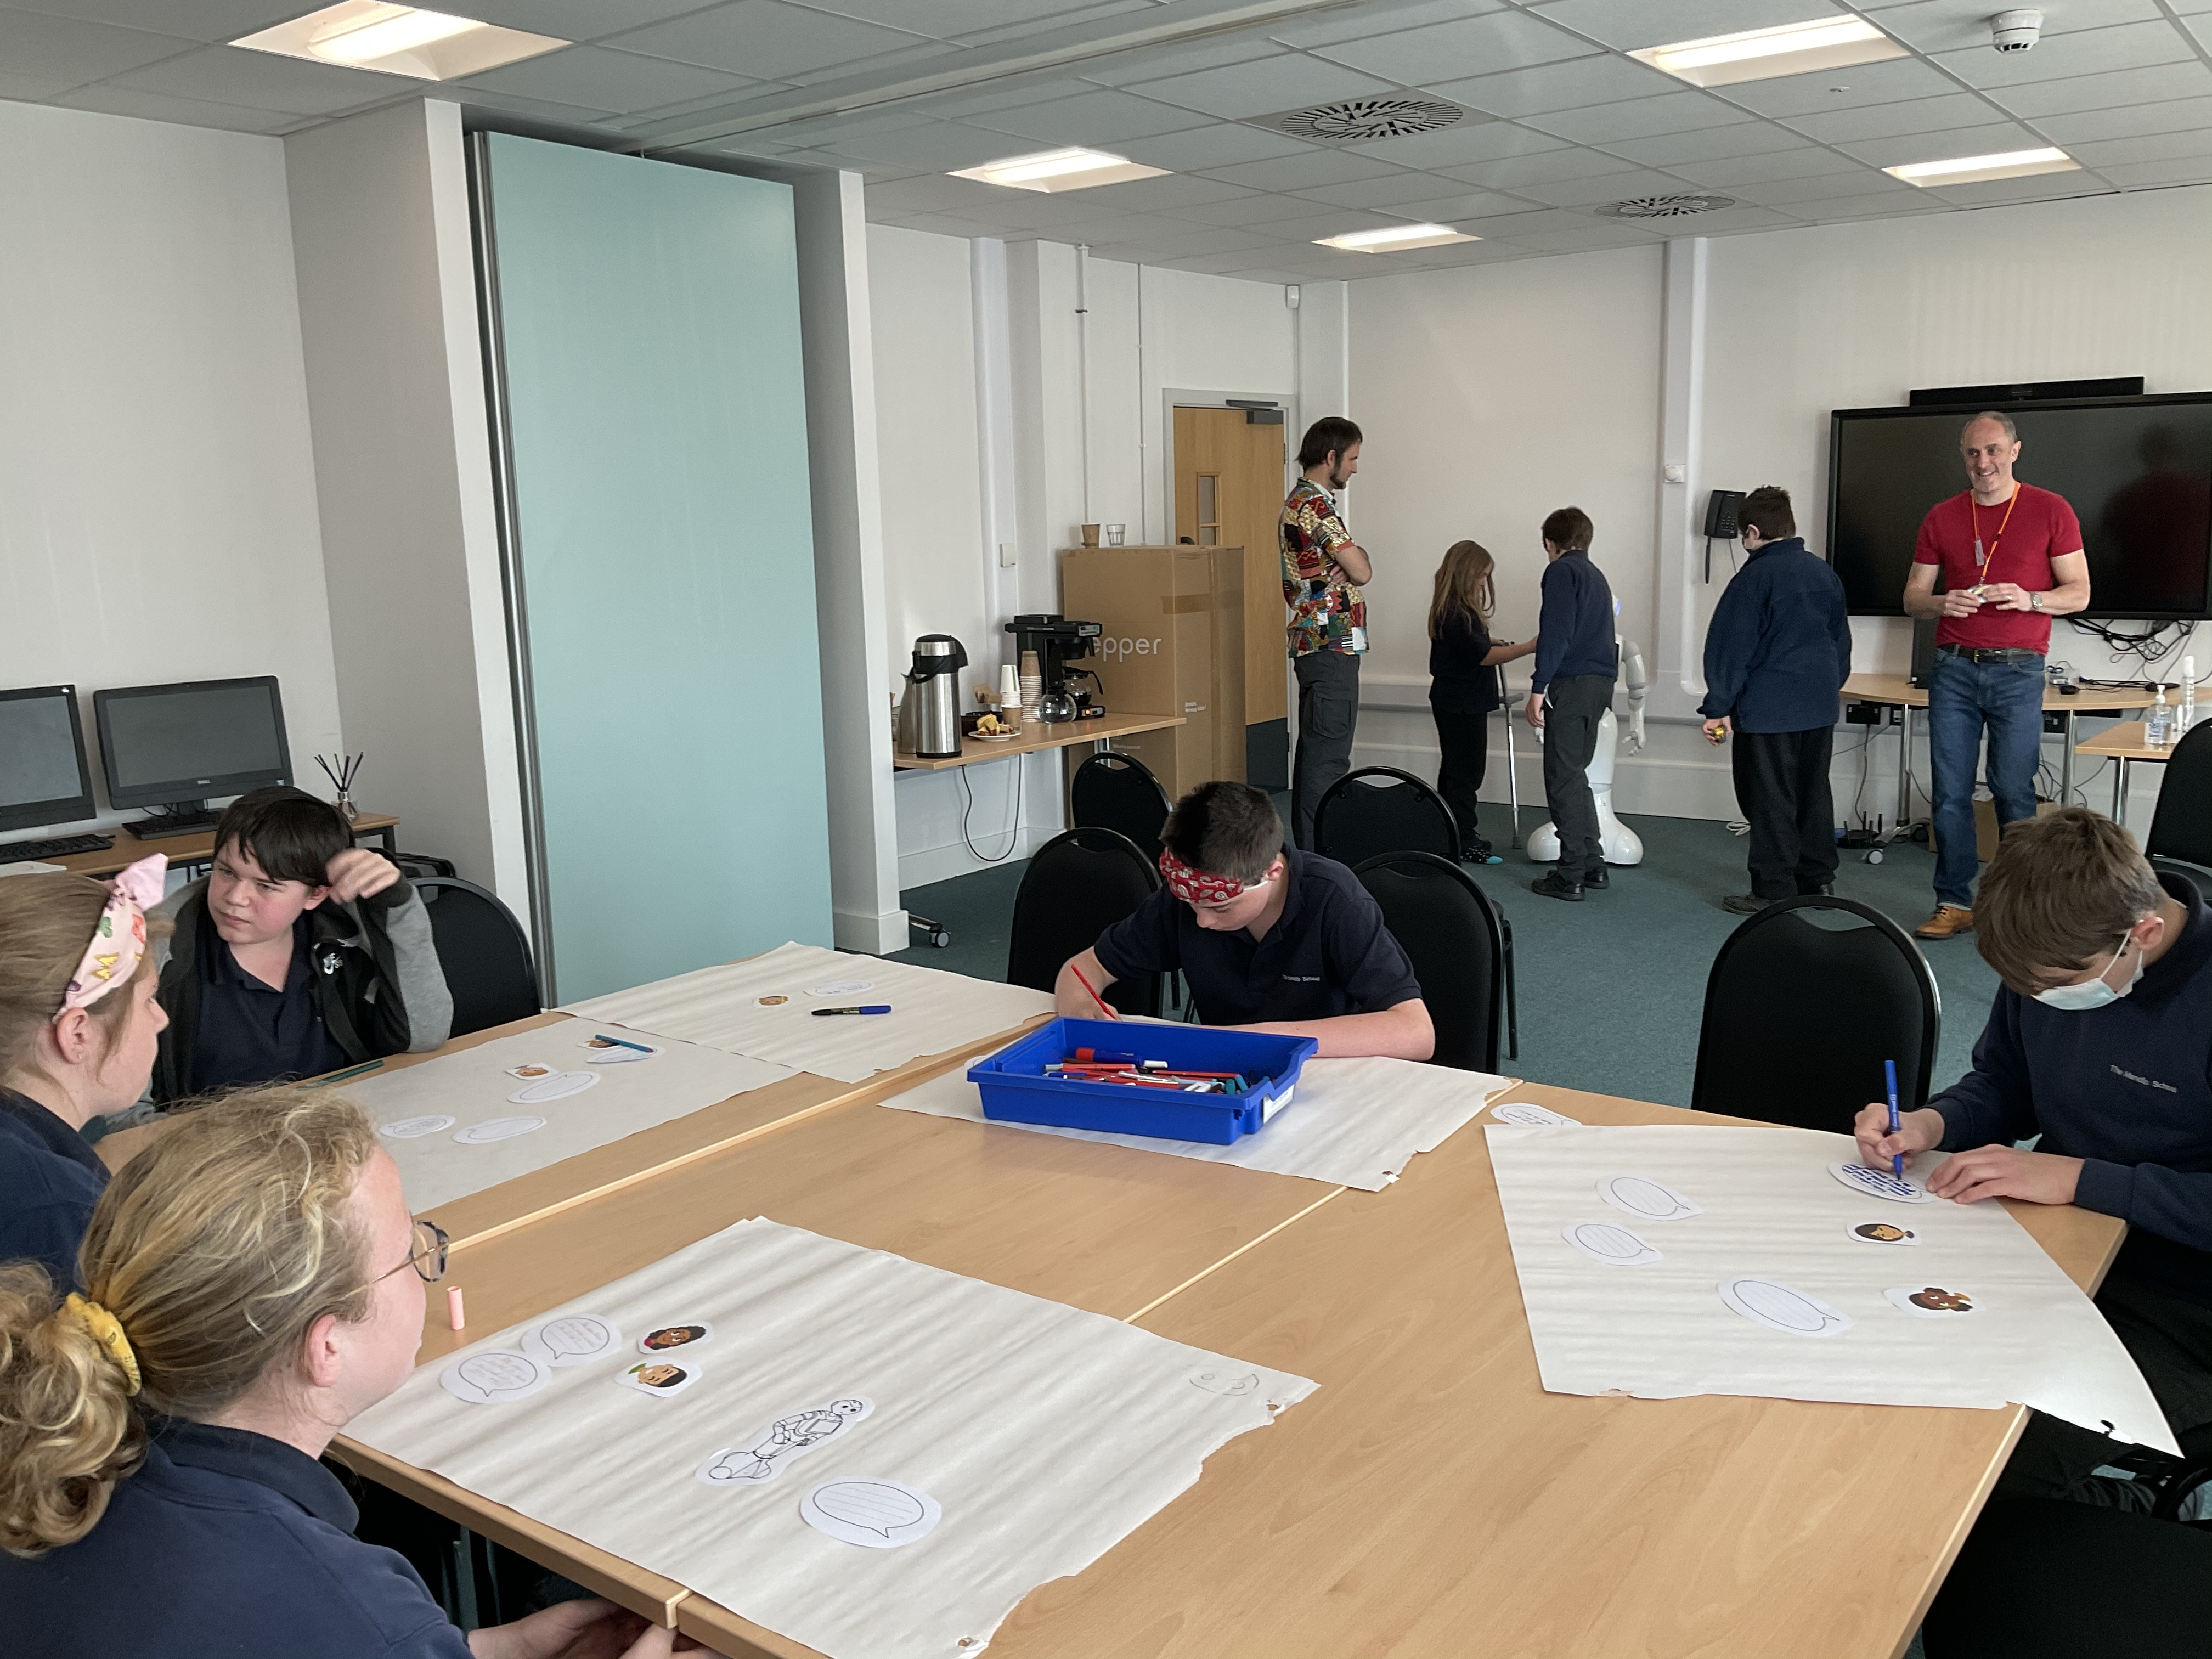
\includegraphics[width=0.5\linewidth]{figs/robots4sen/image7.jpeg}};
        \end{tikzpicture}

    \end{center}
\end{frame}

\begin{frame}{Engagement over 3 weeks}
    \begin{center}
        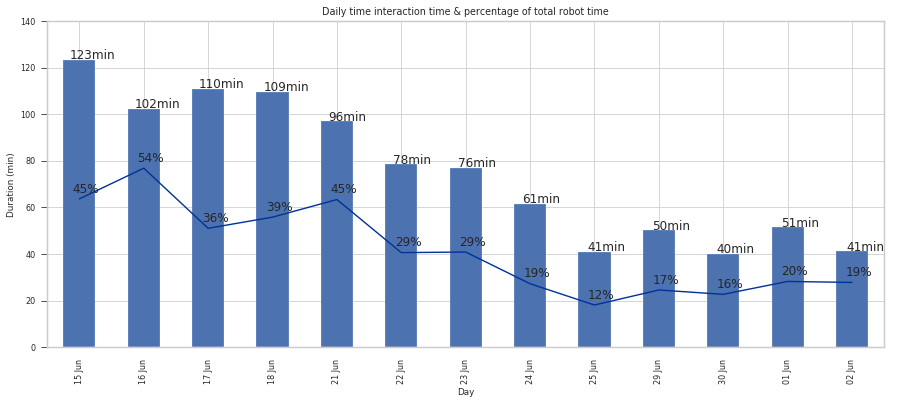
\includegraphics[width=0.8\linewidth]{figs/robots4sen/fig4.png}
        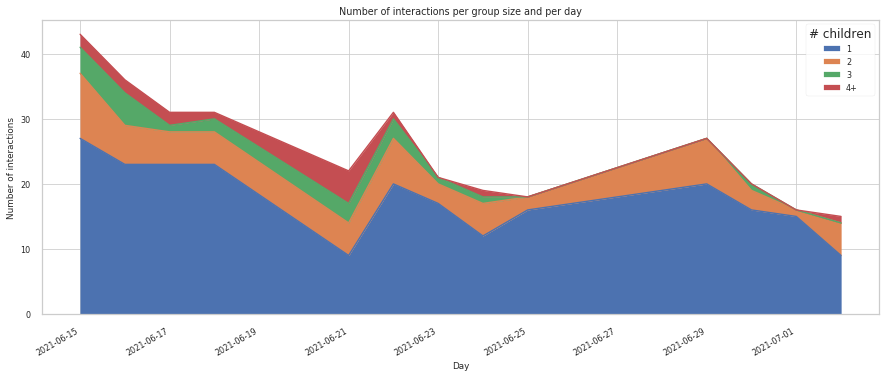
\includegraphics[width=0.8\linewidth]{figs/robots4sen/fig1.2.png}
    \end{center}
\end{frame}


\begin{frame}{Social companions to support children's well-being}
\begingroup
\setbeamercolor{block title}{bg=hriSec2Dark}
\setbeamercolor{block body}{bg=hriSec2}
            \begin{block}{}

                \begin{itemize}
                    \item open-ended, underspecified situations
                    \item  rich semantics
                    \item  complex social dynamics (incl. groups)
                    \item  close the ``interaction loop''
                    \item  sustain long-term autonomous social interactions
                    \item  real-world robustness

                \end{itemize}
            \end{block}
\endgroup

\pause
    \begin{center}
        But limited autonomy! Interactions child-led!

        \pause

        $\Rightarrow$ The next frontier
    \end{center}
\end{frame}

%%%%%%%%%%%%%%%%%%%%%%%%%%%%%%%%%%%%%%%%%%%%%%%%%%%%%%%%

{
    \fullbackground[color=black]{lastpage}
    \begin{frame}[plain]

        \begin{columns}
            \begin{column}{0.6\linewidth}
            \end{column}
            \begin{column}{0.4\linewidth}

                \setbeamercolor{hriSec1Demo}{fg=white!70!black}
                \vspace{6em}
                \begin{beamercolorbox}[wd=\linewidth,ht=6ex,dp=0.7ex]{hriSec1Demo}
                    \textbf{Thank you!}

                    \vspace{2em}
                    \footnotesize
                    Get the slides:\\
                    \href{https://github.com/severin-lemaignan/presentation-codesign}{github.com/severin-lemaignan/presentation-codesign}
                \end{beamercolorbox}
            \end{column}
        \end{columns}
    \end{frame}
}

\appendix
\imageframe[scale=0.9]{pd_comparison}

\end{document}
